\section{Background on Topological Data Analysis}
\label{sec:background}

TDA extracts structural, shape-based features from data that are invariant
to continuous deformations and robust to noise~\cite{cohen2005stability}.
Figure~\ref{fig:placeholder} summarizes the pipeline used in this work:
a metric point cloud is covered by a filtered simplicial complex, from
which persistent homology is computed and summarized as a set of Betti
numbers. We formalize each component below.

\begin{figure}[H]
    \centering 
    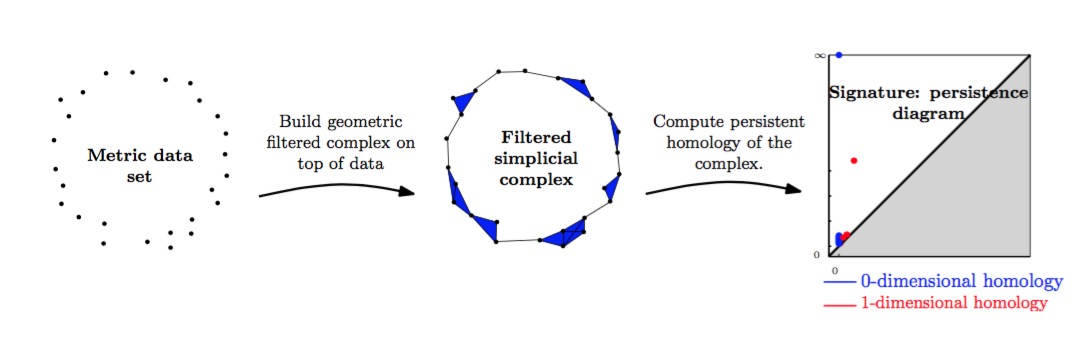
\includegraphics[width=1\linewidth]{imgs/Illustration_of_Typical_Workflow_in_TDA.jpeg}
    \caption{Illustration of a typical workflow in Topological Data Analysis}
    \label{fig:placeholder}
\end{figure}

% ------------------------------------------------------------------
\subsection{Simplicial Complexes, Filtrations, and Homology}
\label{subsec:simplicial}
% ------------------------------------------------------------------

\paragraph{Simplicial complexes.}
A \emph{$k$-simplex} is the convex hull of $k+1$ affinely independent
points: a 0-simplex is a vertex, a 1-simplex is an edge, a 2-simplex is
a triangle, and a 3-simplex is a tetrahedron.
A \emph{simplicial complex} $K$ is a finite collection of simplices
closed under the face relation: if $\sigma \in K$ and $\tau$ is a face
of $\sigma$, then $\tau \in K$.
Figure~\ref{fig:placeholder} illustrates two canonical examples:
a three-dimensional complex (a solid tetrahedron, left) and a
two-dimensional triangulation of a toroidal surface (right). A
\emph{triangulation} decomposes a surface into non-overlapping triangles
such that adjacent triangles share exactly one edge or vertex.
The torus is directly relevant to our setting: the cyclic group
$\mathbb{Z}_{p}$ for $p \in \mathbb{N}$ underlying our arithmetic tasks is embeddable in a
2-torus $\mathbb{T}^2 = S^1 \times S^1$, which constrains the expected homological
structure of the learned representations.

% Side-by-side figures
\begin{figure}[H]
\centering
\begin{minipage}{.45\textwidth}
  \centering
  \includesvg[width=0.475\linewidth]{imgs/Simplicial_complex_example.svg}
  \captionof{figure}{Three dimensional Simplicial Complex, because its higher simplex has dimension 3, which is the tetrahedron.}
  \label{fig:test1}
\end{minipage}\hfill
\begin{minipage}{.45\textwidth}
  \centering
\includesvg[width=0.475\linewidth]{imgs/A_triangulation_of_the_torus,_with_bounding_box_fixed.svg}
  \captionof{figure}{A triangulation can be understood as a two dimensional Simplicial Complex, since its higher dimensional simplex are triangles. }
  \label{fig:test2}
\end{minipage}
\end{figure}

\paragraph{Filtrations.}
Given a set $X = \{x_1, \ldots, x_n\} \subset \mathbb{R}^D$,
a \emph{filtration} constructs a nested sequence of simplicial complexes
\begin{equation}
    \emptyset = K_0 \subseteq K_1 \subseteq \cdots \subseteq K_m = K
    \label{eq:filtration}
\end{equation}
indexed by a non-decreasing scale parameter $\varepsilon_0 \leq \cdots
\leq \varepsilon_m$. In the \emph{Vietoris--Rips} construction,
$\{x_{i_0}, \ldots, x_{i_k}\}$ spans a $k$-simplex at scale $\varepsilon$
if and only if all pairwise distances are at most $\varepsilon$. As
$\varepsilon$ grows, isolated points are connected into edges, triangles,
and higher simplices, as depicted in Figure~\ref{fig:placeholder}
(center). For small $\varepsilon$ the complex is disconnected; for large
$\varepsilon$ all topology collapses into a single contractible component.
In our pipeline we use an adaptive $k$-nearest-neighbor variant, where
an edge $(x_i, x_j)$ is included if their distance falls within the
95th percentile of distances to the $k$-th nearest neighbor across $X$.

\paragraph{Homology and Betti numbers.}
The \emph{boundary operator} $\partial_k : C_k \to C_{k-1}$ maps each
$k$-simplex to the formal sum of its $(k-1)$-faces, satisfying
$\partial_{k-1} \circ \partial_k = 0$. The \emph{$k$-th homology group}
\begin{equation}
    H_k(K;\,\mathbb{Z}_2) \;=\; \ker(\partial_k)\,/\,\mathrm{im}(\partial_{k+1})
\end{equation}
isolates $k$-dimensional cycles that do not bound any $(k+1)$-dimensional
region. The \emph{$k$-th Betti number} $\beta_k = \mathrm{rank}(H_k)$
counts these independent holes: $\beta_0$ counts connected components,
$\beta_1$ counts independent loops, and $\beta_2$ counts enclosed voids.
For example, the tetrahedron and torus in Figure~\ref{fig:test1} and~\ref{fig:test2},
the Betti vectors are $(1,0,1)$ and $(1,2,1)$ respectively, confirming that these invariants capture the qualitatively different topological
structure of the two shapes. 


\subsection{Intrinsic Dimension Estimation}
\label{subsec:id}
% ------------------------------------------------------------------

The \emph{intrinsic dimension} (ID) of $X \subset \mathbb{R}^D$ is the
minimum $d$ such that $X$ lies approximately on a $d$-dimensional smooth
manifold, independently of the dimension $D$. We estimate ID using the Maximum Likelihood Estimator of Levina and
Bickel~\cite{LevinaBickel}, where given distances $r_1(x) \leq \cdots
\leq r_k(x)$ from $x$ to its $k$ nearest neighbors,
\begin{equation}
    \hat{d}_k(x) = \left[
        \frac{1}{k-1} \sum_{j=1}^{k-1}
        \log \frac{r_k(x)}{r_j(x)}
    \right]^{-1},
    \label{eq:mle_id}
\end{equation}
with the global estimate obtained by averaging over all $x \in X$. 

We use $\hat{d}_k$ for two purposes in our pipeline. First, as a geometric descriptor tracked over training (Section~\ref{subsec:results_id}). Second, as the target dimension for dimensionality reduction prior to persistent homology computation: activation matrices are reduced to $\mathbb{R}^{2\hat{d}}$ via UMAP~\cite{McInnes2018}, motivated by the Strong Whitney Embedding Theorem~\cite{whitney1944self}, which guarantees the existence of a smooth embedding of any $d$-dimensional manifold into $\mathbb{R}^{2d}$. The resulting Betti numbers should be interpreted as indicative of structural trends rather than exact invariants. %We return to this limitation in Section~\ref{subsec:conclusion_limitations}.

\begin{theorem}[Strong Whitney's Embedding Theorem \cite{whitney1944self}]
    Any smooth real $m$-dimensional manifold (required also to be Hausdorff and second-countable) can be smoothly embedded in the real $2m$-space, $\mathbb{R}^{2m}$, if $m > 0$. 
\end{theorem}